\chapter{Model development}
\label{chap:ModelDevelopment}
This chapter will discuss the simulation model used for the evaluation of the option pricing techniques. \todo{descr} 

\section{Simulation model}
\label{sec:SimulationModel}
In this thesis, a series of simulations will be run to determine the performance of different option valuation models. These pricing models range from theoretical optimal --- the all knowing seller --- up till the practically implementable --- based upon historical prices and Monte~Carlo simulation.

The first simulation run will determine the maximum possible profits an option seller could ever realize. The results will be acquired by assuming an option writer that has perfect information and acts accordingly. Because this model yields the absolute maximum a seller could never gain more from offering lock-in product, the observations of this run will also be used as the baseline to compare the performance of other option models with.

The runs after the optimal case will drop some of the assumptions made about the all knowing seller, and determine the influences of those assumptions on the results. The final case will be a practically implementable option valuation model based upon historical prices.

To determine the outcomes associated with each of the models, each simulation will run through a number of steps. This process is illustrated in \autoref{fig:simulationProcess}. The processes above the line are the ones connected to the buyer, while the ones below are linked to the airfare~lock-in product seller.

\insertfigure{simulationProcess}{Illustration of simulation process}

The process illustrated in the figure can be described in more detail using the seven~consecutive steps:

\begin{description}
\item[Arrival of passenger] In the first stage of the simulation, the model will generate the arrival of passengers. A passenger is interested in buying on airfare~lock-in product on a specific flight. In this research, the model will generate a single passenger for each day prior to departure of a specific flight. Because data have been collected on flights up till 42~days before departure, each ticket will receive this same number of passengers with option requests. However, because when selling options with a specific number of days to maturity $m$ it is not possible to buy options fewer that $m$ days to departure, these customers get excluded from the model. As an example, the test dataset containing airfares of tickets from LHR to JFK includes 7,690 unique flights after cleansing. When simulating this model for options with a maturity of 3 days a total of $(42 - 3) \times 7,690 = 299,910$ passengers will be generated.

\item[Calculate the passenger's WTP] The next step of the simulation will engage itself in the calculation of the customer's Willingness To Pay. This amount is determined by computing the minimum of the expected utility of buying the flight immediately, or postponing the decision to fly $m$~days later.

The exact level of a customer's WTP is dependant on three other variables. These variables are \begin{inparaenum}[\itshape (i)\upshape]
    \item the customer's forecast of the expected increase in airfare,
    \item the overestimation factor, and
    \item likelihood of travelling.
\end{inparaenum} The implementation of these concepts is explained in detail in \todo{ref}.

Now that the customer knows his level of WTP, he requests the seller for the price of the option.

\item[Calculate the option seller's WTA] The third step is responsible fo the computing the option seller's minimum \emph{Willingness To Accept}. A writer's WTA is the minimum level at which the seller wants to offer options that insure against price risks. When he would offer the airfare~lock-in products at this value, the seller would not expect any returns on the sale. The WTA of the external party is thus calculated using the writer's predictions of how the airfare is expected to change.

The simulation model in this thesis uses many different configurations of option sellers. In the first case, a lock-in product seller with perfect information is considered. The exact configuration of this entity will be described in detail in \todo{ref}.

\item[Calculate the price of the option] Step number four will calculate the price at which the option will be offered to the passenger. This simulation will calculate this value by either setting it to the customer's exact degree of WTP, or by applying a margin on top of the WTA calculated in previous step. The customer then gets offered the option at the computed price.

\item[Acceptance of the offer] The next step will determine whether the customer will accept the airfare~lock-in product offer. This is done by comparing the customer's WTP and the offered option price. When the Willingness To Pay of the customer for a certain flight is higher than the option price calculated in prior process, a customer will accept the offer (i.e., $\text{WTP} \ge p_O$).

\item[Exercising the option] The second-last step in the simulation process will determine whether the customer will actually exercise his option at the date of maturity. To do so, the model will first `wait' $m$~days, and check the observed ticket price. A customer will only exercise its right when this observed airfare is higher than the strike price of the option, $p_S$. Furthermore, the passenger will only use the option when he has decided to fly. When both of these rules apply to a certain customer, he will thus make use of his lock-in product, and let the seller buy the flight ticket for him.
    
\item[Calculate geneterated outcomes] The final step in the model will calculate the outcomes of each sold option. When the customer does not exercise his option on the date of maturity, the seller thus will gain the full price at which he has sold the option in profits. When the passenger actually does exercise his right, the profits or losses gained from selling the option can be defined as:
$$ y = p_O - (p_S - p_m) $$
\end{description}

Using the method described above, the simulation will be used to compare the performance of the proposed option valuation models. The same procedure will also be used to test the influence of a particular configuration of parameters within a single option valuation model.


\subsection{Parameters and assumptions of the simulation model}
For this simulation, a number of parameters have been defined. The next section will describe these variables, and define the configuration for the baseline which is being used for the initial simulation. The simulation models in later sections (e.g., \todo{ref}) will loosen the specified parameters to see its effects on the performance of the parameters itself.

In this research, a parameter is defined as a variable of the underlying object which can be altered to represent different values. The sensitivity analysis will thus adjust some of these parameters, and determine their influence. For example, the number of days till maturity of an airfare~lock-in product can hold the values 3, 7, 14, or 21~days for different simulation runs.

An assumption is defined as a statement about an entity, which is either true or false. For example, the baseline model of the simulation assumes that the option writer knows the exact level of a customer's Willingness To Pay. In the more practical simulations of option sellers, this assumption is released. In these models the seller does not know the precise value of the passenger's WTP. A release of an assumption in the simulation model thus implies a different option valuation technique.


Like in \typenameref{sec:Entities}, this research will categorize the parameters and assumptions according to their underlying entities. These four sections are \begin{inparaenum}[\itshape (i)\upshape]
\item the flight~ticket,
\item the airfare~lock-in product,
\item the option seller, and
\item the passenger.
\end{inparaenum} Each of these entities has its own set of characteristics, which will be defined below.

\subsubsection{Characteristics of the flight ticket}
\label{sub:CharacteristicsOfTheFlightTicket}
The first entity represents the ticket for a flight. A ticket gives its holder the right to take a seat on a particular underlying flight. In this thesis, a specific set of flights is being used:

\begin{compactitem}
\item each flight is for a specific route between outbound and inbound airport;
\item only single-legged (direct) flights are being considered;
\item only round trip flights are being considered;
\item each flight has a specific departure date;
\item the return date of the flight is always 1~week after the departure date.
\end{compactitem}

\vspace{1em}

Each ticket also has a certain price. This price can differ depending on the lookup~time of the ticket. In this research, airfare changes have been monitored up to six~weeks (i.e., 42~days) prior to departure. A certain price of a ticket can thus be defined in the number of \emph{days before departure}, or \emph{dbb}.

This thesis has collected airfares on flight tickets for 22~different routes during a period of 12~weeks. The empirical data acquired in this stage are being used in the simulation model. The complete analysis on these airfares is given in \autoref{chap:DataAnalysis}.

\subsubsection{Characteristics of the airfare~lock-in product}
The next entity which is being considered in this simulation model is the airfare~lock-in product. This product gives its holder the right --- but not the obligation --- to buy the underlying flight. There are two parameters associated with the entity.

\parameter{the option's number of days till maturity \hfill ($m = 3$)}
The first parameter of the airfare~lock-in products is its number of days till maturity. This value denotes the number of days of extra \emph{decision time} a customer gains when he buys the option. At the date of maturity, the customer has to make the decision to actually buy the ticket, or to not exercise the option at all. A passenger will choose for the first alternative when he has decided to actually fly, and the current airfare is higher than the agreed upon \emph{strike price}. During this number of days $m$, the customer is thus \emph{insured} against price fluctuations and will therefore not risk high fare increases.

In the baseline model of the simulation, a maturity of 3~days is being considered. When a passenger thus purchases the option, he will decide whether to exercise the option 3~days after the acquisition of the lock-in product.

\parameter{the option's strike price \hfill ($p_S = p_I$)}
The second parameter associated with the entity is the strike price of the airfare~lock-in product. This price, denoted by $p_S$, is the cost at which the passenger is able to buy the underlying flight ticket when he exercises the option.

This research will consider a strike price of the airfare~lock-in product that is equal to the initial airfare of the underlying flight at purchase of the option.
$$p_S = p_I$$

For example, when the current ticket price $p_I$ is equal to \$\,100 and the customer decides to buy the option, he has the opportunity to buy the ticket for \$\,100 at the date of maturity.  

Next to these configurable parameters, an airfare~lock-in product also has a certain price at which the option is offered to the customer. The theoretical level of this option price is described in \typenameref{subsec:PassengersWTP}. In this research, however, a number of different option valuation techniques are being considered. These pricing models are characterized by different configurations of the parameters of this simulation model, and will be described in detail in \autoref{chap:Results}.


\subsubsection{Characteristics of the options seller}
Another entity considered in the simulation model of this research is the seller of the airfare~lock-in products. This is the object that offers the options to the customer. The simulation model described also has associated some parameters and assumptions to this entity.

As stated previously, the first simulation model built for this research is assuming an option seller with perfect information. This theoretical case will provide insights into the maximum possible profits a writer can achieve. Furthermore, this model is also valuable as baseline to compare other option models with. This section will describe the exact assumptions and parameters that are associated with this entity.

To the seller with perfect information, a number of assumptions apply:

\assumption{the seller knows the exact price movements of tickets}
The first assumption states that the seller knows the exact fare fluctuations of the underlying flight ticket. He thus has foreknowledge which enables him to make 100~percent accurate forecasts. By doing so, the writer will be able to set a minimum option price which ensures no losses when the option is exercised.

This characteristic thus supports the seller in setting a minimum option price. When this amount would be used, the seller would not make any profits when the passenger decides to exercise the product. The maximum price an option seller can set is determined by the customer's Willingness To Pay. This is where the next assumption of the all knowing seller comes in.

\assumption{the seller knows the exact level of a customer's Willingness To Pay}
The second assumption states that the seller with perfect information also knows the exact level of the passenger's Willingness To Pay. This allows the writer to set its option prices at the highest level at which the customer still accepts the offer.

\assumption{the seller knows whether the customer will exercise its option at maturity}
The third assumption defines that the option seller knows at the beginning of the simulation procedure whether the customer will actually exercise its right at the date of maturity. A seller will use this information to set the lowest Willingness To Accept for each customer. For example, when the seller knows the customer will \emph{not} exercise his option, the writer can make profit on any offer to a customer whose WTP is higher than $0$.

On the other hand, when the seller knows the passenger \emph{will} exercise his option on the date of maturity, the minimum WTA of an option should equal the expected costs. In this model that is characterized by a seller with perfect information, these `costs' can be evaluated at $0$, because of the fourth assumption.

\assumption{the seller will buy tickets in advance when he knows the passenger will fly and airfare increases}
The fourth assumption of the seller with perfect information states that the seller is able to buy tickets in advance. Combined with the first assumption that the writer can make 100~percent accurate forecasts of ticket prices, and the third assumption that he knows whether the customer will decide to fly, he can purchase the flights in advance at the lowest costs. For example, consider that a customer buys an option for a flight of which the current ticket price is $100$. At the date of maturity the airfare has increased to $110$, and the customer decides to fly. Normally the option seller would buy the ticket at the price at maturity, $110$, which results in an increased cost of $10$. However, because the seller with perfect information knows both of these facts on the date he offers the option to the customer, he is able to buy the ticket in advance at the lowest price possible. In this case, the writer would thus buy the ticket at the initial price of $100$, and sell this ticket to the customer at maturity for the strike price. Because the strike price in this simulation model is defined in as the initial airfare, the writer will sell the flight for $100$ to the customer, at which no extra costs incur.

This process of buying tickets in advance is also known as \emph{long selling}. Long selling enables the option writer to buy tickets in advance at the lowest fare possible.

As stated before, these assumptions only apply to the baseline model which simulates an option seller with perfect information. Other runs of the simulation will release some of these assumptions to represent a more practically feasible model. The effect of the assumptions is than quantified by comparing the outcomes to this baseline model.


\subsubsection{Characteristics of the passenger}
The final entity considered in the baseline model for the simulation is the passenger. This passenger doubts whether he will fly on a specific date, and considers to purchase an option which will allow him more decision time. To be able to make this decision, a number of parameters are being considered. These variables together represent the equation which defines the passenger's Willingness To Pay:
$$\mbox{WTP} = \min((1 - P^f) \times p_I, P^f \times E_{p_t} \times \mbox{OEF})$$

The first part of the equation represents the utility of buyting the flight immediately. The second part defines the expected of waiting.

The formula uses a number of characteristics of the passenger: $P^f$ is the likelihood of travelling, $p_I$ represents the initial ticket price, $E_{p_t}$ is the expected increase of the ticket price, and $\mbox{OEF}$ is the overestimation factor. The parameters will be described in this section.

\parameter{the passenger's likelihood of travelling \hfill ($P^f = U(0,1)$)}
The passenger's likelihood of travelling represents the probability of the passenger actually wanting to buy a flight ticket at the time of maturity. This parameter $P^f$ is a value between $0$ and $1$, which represent \emph{certainly \textbf{not} flying} and \emph{certainly flying} respectively. The probability of flying is heterogeneous amongst different passengers, and will be randomly drawn from a uniform distribution, $P^f = U(0,1)$. This thus implies that the average $P^f$ of all the passenger's aggregated is $0.5$. At the time of computing the passenger's WTP, the passenger \emph{does} know the exact value of this variable. The option seller, however, does \emph{not} have this information.

Whether the passenger actually decides to fly at maturity is simulated by drawing another random variable from a uniform distribution $r^f = U(0,1)$. When $r^f \le P^f$ the passenger decides to fly, and when $r^f > P^f$ he decides not to do so. Whether the passenger actually wants to exercise the option thus depends on the outcome of this simulation, and whether the strike price $p_S$ is lower than the airfare at maturity (i.e., $p_S < p_{t+m}$).

\parameter{expected increase in airfare \hfill ($E_{p_t} = 6.55\% \times p_I$)}
Like the seller, the passenger also uses a certain mechanism to make predictions of the airfare at time of maturity. Throughout the simulation model, the passenger will use historical prices to make his own forecast. These data come from the training set acquired during the data collection phase (see \todo{ref}).

A passenger uses the observed historical price increases to determine the expected price fluctuation for a certain flight. This expected increase is dependent on the number of days till maturity of the airfare~lock-in product. For a single flight the expected increase can be defined as:
$$E_{p_t} = 1 - \frac{p_{t+m}}{p_t}$$

The exact level of expected increase is homogeneous for all passengers, and determined by the average price increase of all routes for all number of days before departure. \autoref{tbl:ExpectedIncreases} gives the expected price fluctuations associated with each number of days till maturity.


\begin{table}
\centering
\footnotesize
\begin{tabular}{l c}
    \toprule
    $m$       &  $E_{p_t}$ \\
    \midrule
    3         &   6.55\,\%  \\
    7         &  14.93\,\% \\
    14        &  29.39\,\% \\
    21        &  44.06\,\% \\
    \bottomrule
\end{tabular}
\caption{Expected increase of airfare}
\label{tbl:ExpectedIncreases}
\end{table}


\parameter{overestimation factor \hfill (\mbox{OEF} = 100\%)}
The last parameter that influences the price is the overestimation factor of a passenger (i.e., $\mbox{OEF}$). A overestimation factor higher than $100\,\%$ mean the passenger overestimates the expected increase in price, while one lower will represent a customer that underestimates the future ticket price. This factor thus somewhat represents the risk aversion of a passenger by letting it increase or decrease his Willingness To Pay by a certain amount. The parameter will be used in the sensitivity analysis part of the simulation to see what overestimation has on the outcomes of the model.


To illustrate the whole process of calculating a customer's WTP, consider a passenger that wants to buy an option on a flight with a $p_I$ of $100$. The customer is characterized by a randomly generated $P^f$ of $0.25$, and an $\mbox{OEF}$ of $100\%$ (i.e., risk neutral). The utility of buying the flight immediately is 
$$\mbox{WTP}_{buy} = (1 - 0.25) \times 100 = 75$$

When the customer wants to buy extra decision time of 3~days (i.e., $m = 3$), his WTP for waiting would be
$$\mbox{WTP}_{wait} = 0.25 \times E_{100} \times 100\% = 0.25 \times (100 \times 0.0655) \times 100\% \approx 1.64$$

The actual customer's $\mbox{WTP}$ will thus become the minimum of both utilities:
$$\mbox{WTP} = \min(\mbox{WTP}_{buy}, \mbox{WTP}_{wait}) = \min(75, 1.64) = 1.64$$


\subsubsection{General characteristics of the simulation model}
Next to the parameters and assumptions specific to the four entities described previously, the simulation model itself also has some characteristics defined.

\parameter{arrival rate of passengers \hfill ($(42 - m) \times n$)}
As seen in the process description of the simulation (see \todo{ref}), the model will generate passengers to determine the performance of the model. A passenger will arrive at every day before the departure of the flight for the full observed 42~days. However, it is only possible for a passenger to buy an option with $m$ days to maturity up till $m$ days before departure. The number of customer arrivals per flight is thus fixed per simulation and can be expressed as $42 - m$.

For each specific route with $n$ flights, the simulation will therefore generate $(42 - m) \times n$ passengers.

\parameter{number of trials \hfill (N=150)}
Because pseudo random generation of numbers and probabilities are used in this model, there is a possibility of generating outliers in only a single run. To prevent such scenarios from happening, every simulation is run a vast amount of times. The acquired data from these multiple trials is then averaged to get the converged mean.

\todo[The convergence plot of three example flights is shown in \autoref{fig:ConvergencePlotMultiple}. As can be seen in the figure, the mean seems to stabilize at around 150~trials. This research will therefore use the average of 150~trials for every simulation.]{new}

%\begin{figure*}
%\centering
%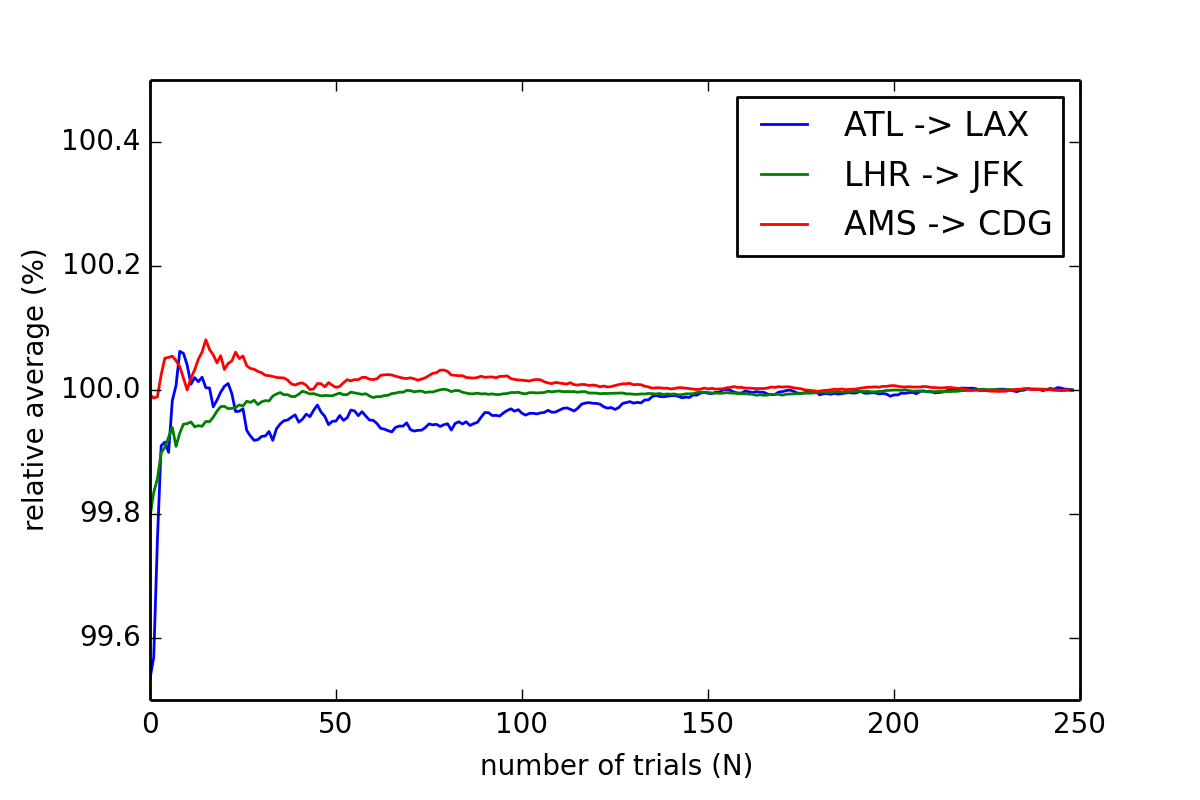
\includegraphics[width=0.6\textwidth]{figures/ConvergencePlot_multiple}
%\caption{Convergence plot}
%\label{fig:ConvergencePlotMultiple}
%\end{figure*}
